\section{Introduction}

	Le cas étudié porte sur "la gestion des contacts commerciaux" d'une banque. Les applications à concevoir et l'architecture du poste de travail doivent apporter une aide aux agents commerciaux.

\section{Livrables}

Tout au long du projet, des livrables bien définis doivent être fournis aux clients. L’objet de cette partie est de décrire le rôle et le contenu de chacun des ces livrables.
\subsection{Phases}

Pour Chaque phase, nous préciserons son but, son déroulement et le(s) livrable(s) attendu(s). Les phases de notre étude préalable sont les suivantes :

\subsubsection{Initialisation}

\paragraph{Buts}
\begin{itemize}
    \item Cibler le champs d’étude du projet
    \item Identifier les contraintes et risques
    \item Élaborer notre démarche
\end{itemize}


\paragraph{Déroulement}
\begin{description}
    \item[Contexte général]{
        Il s’agit de faire une introduction présentant brièvement l’entreprise, l’état du service existant, ainsi que notre rôle dans ce projet.
    }
    \item[Livrables]{
        Il s’agit d’élaborer une liste exhaustive des livrables.
    }
    \item[Mode opératoire et phasage]{
        Il s’agit de choisir les méthodes à adopter, découper le projet en plusieurs phases.
    }
    \item[Activités / taches]{
        Il s’agit d’identifier les taches et activités de chaque phase, les répartir entre les différents collaborateurs selon un planning prévisionnel.
    }
    \item[Organisation de l’équipe]{
        Il s’agit de définir le rôle de chaque membre ainsi que ses principales missions au sein du projet.
    }
    \item[Analyse des risques]{
        Il s’agit de faire une analyse prévisionnelle des risques liés au projet et élaborer un plan de gestion de ces risques.
    }
\end{description}

\paragraph{Livrables}
Dossier d’initialisation

\subsubsection{Conception d'ensemble}

\paragraph{But}
\begin{itemize}
    \item Identifier les évolutions de l'architecture applicative, nécessaires pour satisfaire les besoins des utilisateurs.
\end{itemize}


\paragraph{Déroulement}
\begin{description}
    \item[Diagrammes d'activité]{
        Effectuer un découpage des cas d'utilisation représentatifs en scénarios élémentaires et spécification de ces scénarios sous forme de diagramme d'activité
    }

    \item[Découpage MCD et définition des blocs]{   
		Il s'agit de découper le MCD en blocs applicatifs et de définir ces différents blocs}

    \item[Dynamique de l'architecture : diagrammes des séquences]{
		A l'aide des différents blocs applicatifs, il faut créer les diagrammes de séquences découlant des diagrammes d'activité}
	\item[Dynamique de l'architecture : diagrammes de collaboration]{
		Le diagramme de collaboration est la phase finale qui découle des diagrammes de séquence. Il s'agit de représenter les différents échanges entre blocs applicatifs}
	\item[Architecture générale]{
		L'architecture générale doit définir une première architecture vue globalement}
	
\end{description}

\paragraph{Livrables}
\begin{itemize}
    \item Dossier de conception d'ensemble
\end{itemize}

\subsubsection{Conception détaillée}

\paragraph{Buts}



\paragraph{Déroulement}
\begin{description}
    \item[EDF et IHM]{
        Création des EDF et IHM pour chaque objet métier (Contact, Client, Agenda)
    }
	\item[Liste des services]{
        Création des listes de services pour chaque objet métier (Contact, Client, Agenda)
    }
	\item[Spécification Service Métier et Service Objet Métier]{
    }
\end{description}

\paragraph{Livrables}
\begin{itemize}
    \item Dossier de conception détaillée
\end{itemize}

\subsubsection{Architecture technique}

\paragraph{Buts}

\paragraph{Déroulement}
\begin{description}
	\item[Spécification de l'architecture technique volet production]{
		topologie réseau, implantation des composants du noyau applicatif et spécification des flux applicatifs
    }
\end{description}
\paragraph{Livrables}
\begin{itemize}
    \item Architecture Technique
\end{itemize}


\section{Identification des activités et des tâches}
Le tableau suivant rend compte du temps et des ressources alloués à chaque tâche. Il s'agit d'un planning prévisionnel qui peut être contraint au changement.

    \begin{center}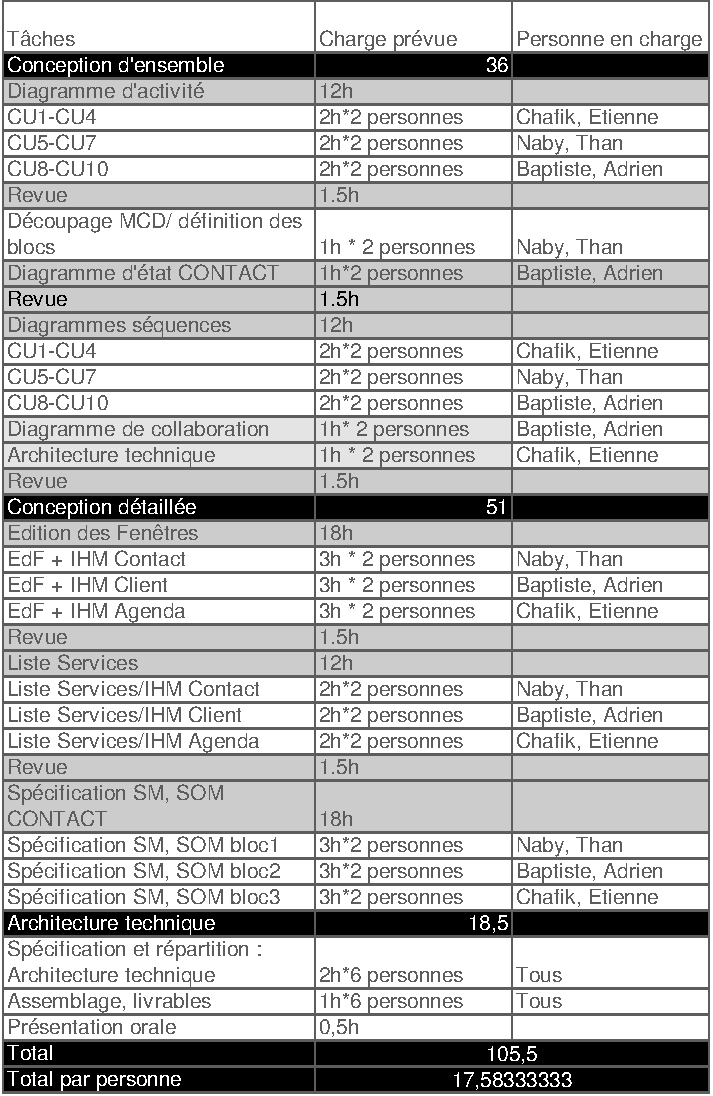
\includegraphics[height=0.6\textheight]{h4212SuiviTache.png} \end{center}

\vspace{10 mm}

\section{Suivi}

Le suivi des tâches s'effectue sous la plateforme RedMine. Chaque tâche y est définie (Description, temps prévu, ressources alloués). Chaque membre de l'équipe se doit d'indiquer les tâches qu'il a terminer en n'oubliant pas de 
renseigner le temps passer dessus. Il sera ainsi possible en fin de projet de voir la différence entre le temps prévu et le temps réalisé.

\section{Organisation de l'équipe}

L’équipe projet sera organisé ainsi :
\subsection{Chef de projet : Baptiste \textsc{Lecornu}}

Son rôle sera :
\begin{itemize}
    \item Suivi stratégique du projet
        \subitem Évaluation des risques
        \subitem Respect des objectifs
        \subitem Respects des délais
    \item Pilotage opérationnel
        \subitem Planification des taches
        \subitem Suivi et encadrement des tâches
    \item Organisation humaine
        \subitem Définition du rôle des membres et leur responsabilité
        \subitem Résolution de conflits et arbitrage
    \item Pilotage de la production
        \subitem Suivi des résultats et livrables
        \subitem Méthodes et outils
    \item Production des livrables
\end{itemize}

\subsection{Membres de l'équipe : Chafik \textsc{Bachatene}, Adrien \textsc{Brochot}, Etienne \textsc{Brodu}, Naby Daouda \textsc{Diakite}}

\section{Analyse des risques}
\subsection{Risques}

\newcounter{risques}
\setcounter{risques}{0}

\newcommand{\risque}[1]{
    \addtocounter{risques}{1}
    \item[R\therisques]{\indent#1}
}
Les risques sont les suivants :
\begin{description}
    \risque{Risque humains (liés aux compétence, absence, maladie..)}
    \risque{Apparition de tâches supplémentaires liées à la saisie des livrables ( rapport)}
    \risque{Difficulté d’évaluation du temps nécessaire à chaque tâche(prise en main des outils et méthodes utilisés,...)}
    \risque{Spécification incomplète des points à traiter}
    \risque{Risque de sur-qualité}
    \risque{Délais tendus}
    \risque{Demande régulière de modification durant l’élaboration des solutions}
\end{description}

\subsubsection{Gestion des risques}

\newcounter{solutions}
\setcounter{solutions}{0}

\newcommand{\solution}[1]{
    \addtocounter{solutions}{1}
    \item[S\thesolutions]{\indent#1}
}

Les solutions que nous préconisons sont :
\begin{description}
    \solution{
        \begin{itemize}
            \item Imposer un certain nombre de règles à suivre pour le bon déroulement du projet et veiller au respect de ceux-ci. Si nécessaire formaliser ces règles sous forme de “règlement intérieur”.
            \item Motiver suffisamment les membres de l’équipe  et répartir les tâches en fonction des profils et des compétences de chacun
            \item Redistribuer le travail du membre indisponible aux autres membres de l’équipe durant toute la durée de son indisponibilité.
        \end{itemize}}
    \solution{
        Prévoir des créneaux horaires (hors séance) pour la prise en main des outils utilisés  et la centralisation de façon efficace des différents livrables.}

    \solution{
        Contrôle du planning prévisionnel et mise à jour de celui-ci et si nécessaire réaffectation des tâches}
    \solution{
        S’adresser au client pour éclaircir les points flous}
    \solution{
        \begin{itemize}
            \item Contrôler de façon permanente l’avancement des tâches et les documents produit
            \item Maquettage
        \end{itemize}}
    \solution{
        \begin{itemize}
            \item Planification détaillée du projet avec un GANTT
            \item Suivi de l’avancement des livrables
        \end{itemize}}
    \solution{
        \begin{itemize}
            \item Seuil d’acceptation des modifications
            \item Report des modifications en fin de projet
            \item Gestion de versions
        \end{itemize}}
\end{description}
